\chapter{HASIL DAN PENGUJIAN}
\vspace{1ex}

\section*{}
Pada bab ini dipaparkan hasil pengujian serta analisa dari de-
sain sistem dan implementasi .Pengujian dilakukan guna mengetahui tingkat kesalahan dan menarik kesimpulan dari sistem yang telah dibuat.

Pada pengujian ini digunakan \textit{Smartphone Android} dengan spesifikasi hardware seperti pada tabel \ref{tabel:4.0}.
\begin{table}[h!]
		\caption{Spesifikasi \textit{Smartphone} yang Digunakan}
	\begin{tabular}{|l|l|}
		\hline
		\textbf{CPU} & \begin{tabular}[c]{@{}l@{}}Octa-core (4x1.8 GHz Kryo 260 Gold \\ \& 4x1.6 GHz Kryo 260 Silver)\end{tabular} \\ \hline
		\textbf{Internal}       & \begin{tabular}[c]{@{}l@{}}32GB 3GB RAM\end{tabular}  \\ \hline
		\textbf{Chipset}          & Qualcomm SDM636 Snapdragon 636 (14 nm)             \\ \hline
		\textbf{OS}     & Android 8.1 (Oreo), upgradable to Android 9.0 (Pie) \\ \hline
		\textbf{GPU} & Adreno 509         \\ \hline
		\textbf{Bluetooth} & 5.0, A2DP, LE         \\ \hline
	\end{tabular}
	\vspace{1ex}
	\caption{Spesifikasi \textit{Smartphone} yang Digunakan}
	\label{tabel:4.0}
\end{table}




\section{Pengujian Rekaman Data Selama 15 Menit}
\vspace{1ex}
Pengujian ini dilakukan untuk menentukan baudrate bluetooth HC-05 yang akan digunakan dan delay yang diprogram pada arduino. Pada pengujian ini dilakukan dengan cara melakukan rekaman data dengan target durasi rekaman adalah 15 menit. Untuk menentukan delay dan baudrate yang akan digunakan maka pada pengujian ini dilakukan percobaan dengan delay dan baudrate yang berbeda-beda. Untuk delay sendiri memiliki 3 percobaan yaitu delay 1 ms, delay 5 ms, dan delay 10 ms. Sedangkan baudrate yang digunakan untuk percobaan terdapat 3 tahap yaitu 9600, 38400, dan 57600. Berikut ini merupakan tabel hasil pengujian rekaman data selama 15 (Tabel \ref{tabel:4.0.0})
\begin{table}[H]
	\caption{Tabel hasil percobaan rekaman data dengan target 15 menit}
	\begin{tabular}{|c|c|c|c|c|}
		\hline
		\multicolumn{1}{|c|}{{\color[HTML]{000000} \textbf{Delay}}} & \multicolumn{1}{|c|}{\textbf{Baudrate}} &
		\multicolumn{1}{|c|}{ \textbf{\textit{Force}}} &
		\multicolumn{1}{|c|}{\textbf{Durasi}} &
		\multicolumn{1}{|c|}{\textbf{Sampling}}  \\
		(ms) &  \textbf{HC-05}  & \textbf{\textit{close}}  & \textbf{dicapai} & \textbf{rate}  \\
		&  &  &   & (sampel/detik)  \\ \hline
		
		10 & 9600 & tidak & 15 menit & 50  \\ \hline
		5 & 9600 & ya & 2 menit & 68  \\
		& & & 58.20 detik & \\ \hline
		1 & 9600 & ya & 4 menit & 90  \\ & & & 22.98 detik & \\\hline
		10 & 38400 & ya & 3 menit & 72  \\ & & & 23.65 detik & \\\hline
		5 & 38400 & ya & 1 menit & 114  \\ & & & 52.64 detik & \\ \hline
		1 & 38400 & ya & 2 menit & 216  \\ & & & 14.68 detik & \\ \hline
		10 & 57600 & ya & 2 menit & 112  \\ & & & 05.98 detik & \\ \hline
		5 & 57600 & ya & 2 menit & 125  \\ & & & 51.81 detik & \\ \hline
		1 & 57600 & ya & 2 menit & 270  \\ & & & 23.52 detik & \\ \hline
		%10 & 115200 & ya & 3 menit & 117  \\ & & & 52.15 detik & \\ \hline
		%5 & 115200 & ya & 1 menit & 139  \\ & & & 42.05 detik & \\ \hline
		%1 & 115200 & ya & 1 menit & 327  \\ & & & 36.90 detik & \\ \hline
		
	\end{tabular}
	\vspace{1ex}
	
	\label{tabel:4.0.0}
\end{table}

Dapat dilihat pada tabel diatas memiliki 5 kolom yaitu Delay, Baudrate HC-05, Force close, Durasi dicapai, dan \textit{sampling rate}. Delay merupakan durasi jeda waktu yang digunakan pada loop arduino. Baudrate HC-05 merupakan kecepatan pengiriman data oleh modul bluetooth HC-05. Force close merupakan kejadian dimana aplikasi menutup dengan sendirinya. Durasi dicapai merupakan lama waktu rekaman yang telah didapat sampai dengan aplikasi force close. \textit{sampling rate} merupakan jumlah data atau sampel yang didapat selama satu detik.

Pada percobaan pertama dilakukan dengan menggunakan delay 10 ms, baudrate HC-05 sebesar 9600, dan frekuensing sampling sebesar 50 data/detik. Pada percobaan pertama berjalan lancar hingga aplikasi dapat merekam data selama 15 menit. Percobaan kedua dilakukan dengan mengubah delay arduino menjadi 5 ms, \textit{sampling rate} yang didapat adalah 68 data/detik, pada percobaan ini aplikasi tertutup dengan sendirinya (\textit{force close}) setelah merekam selama 2 menit 58.20 detik. Percobaan ketiga dilakukan menggunakan delay 1 ms, dengan baudrate tetap sebesar 9600, \textit{sampling rate} yang diperoleh sebesar 90 data/detik, pada percobaan ketiga aplikasi mengalami \textit{force close} setelah merekam selama 4 menit 22.98 detik. Percobaan keempat menggunakan delay 10 ms, dengan baudrate HC-05 diperbesar menjadi 38400, \textit{sampling rate} pada percobaan ini sebesar 72 data/detik, pada percobaan keempat ini aplikasi juga mengalami \textit{force close} setelah merekam selama 3 menit 23.65 detik. Percobaan kelima menggunakan delay sebesar 5 ms, dengan baudrate 38400, \textit{sampling rate} yang diperoleh
sebesar 114 data/detik, dan seperti sebelumnya aplikasi mengalami \textit{force close} setelah merekam selama 1 menit 52.64 detik. Percobaan keenam dilakukan menggunakan delay sebesar 1 ms, dengan baudrate yang sama yaitu 38400, \textit{sampling rate} yang diperoleh sebesar 216 data/detik, aplikasi mengalami \textit{force close} setelah merekam selama 2 menit 14.68 detik. Pada percobaan ketujuh aplikasi juga mengalami \textit{force close}, durasi yang dicapai selama 2 menit 05.98 detik, percobaan ini menggunakan delay arduino sebesar 10 ms, dengan baudrate yang diperbesar menjadi 57600, dan \textit{sampling rate} yang diperoleh sebesar 112 data/detik. Percobaan kedelapan dilakukan menggunakan delay arduino sebesar 5 ms, dengan baudrate sebesar 57600, diperoleh \textit{sampling rate} sebesar 125 data/detik, aplikasi mengalami \textit{force close} setelah merekam selama 2 menit 51.81 detik. Percobaan kesembilan dilakukan dengan menggunakan delay arduino sebesar 1 ms, dengan baudrate sebesar 57600, diperoleh \textit{sampling rate} sebesar 270, aplikasi mengalami \textit{force close} setelah merekam selama 2 menit 23.52 detik. 

Berdasarkan tabel \ref{tabel:4.0.0} dapat dilihat pada kolom \textit{force close} dimana hampir pada semua percobaan yang telah dilakukan mengalami force close pada aplikasi. Apabila dilihat pada kolom durasi dicapai, durasi waktu yang didapat saat aplikasi force close tidak pasti, tetapi sebagian besar aplikasi mengalami force close pada menit ke-2. Sedangkan apabila kolom Force close dihubungkan kolom \textit{sampling rate}
maka aplikasi hanya dapat berjalan dengan baik hingga menit ke-15 dengan menggunakan fruekuensi sampling 50 sampel/detik, untuk frekuensi selain 50 sampel/detik tersebut aplikasi mengalami force close. Berdasarkan analisa maka dapat  semakin besar \textit{sampling rate} yang digunakan maka semakin besar kemungkinan force close pada aplikasi.

Apabila dilihat pada tabel \ref{tabel:4.0} versi \textit{bluetooth} pada \textit{smartphone} adalah versi 5.0. Kecepatan transfer \textit{bluetooth} 5.0 adalah 3 Mbps sedangkan kecepatan bluetooth HC-05 adalah 1 Mbps dan bisa dicustom sampai 1.3 Mbps. \textit{force close} minimal pada \textit{sampling rate} sebesar 68 sampel tiap detik.
Sedangkan sampel tersebut merupakan string yang terdiri dari antara 7 sampai 9 karakter. Apabila dihitung 10 karakter tiap sampel maka aplikasi mengalami \textit{force close} saat menerima data 680 byte tiap detik sehingga masalah \textit{force close} tidak terdapat pada versi bluetooth smartphone yang memiliki kecepatan 3 Mbps dan HC-05 yang berkecepatan 1 Mbps. Setelah dilakukan kaji ulang pada aplikasi kemudian ditemukan masalah penyebab \textit{force close}. \textit{Force close}
terjadi dikarenakan adanya \textit{pop up} pada aplikasi pada saat menerima data, sedangkan \textit{pop up} sendiri memiliki animasi yang berdurasi kurang lebih 1 detik, dilain sisi \textit{pop up} tersebut dipaksa muncul 68 kali dalam 1 detik, sehingga terdapat \textit{pop up} yang bertumpuk pada aplikasi dan menyebabkan \textit{force close}.

Setelah aplikasi tidak mengalami force, dilakukan percobaan
dengan baudrate 57600. Aplikasi dapat melakukan rekaman data
maksimal dengan \textit{sampling rate} sebesar 280 data tiap detik tanpa
mengalami force close. Aplikasi dapat berjalan lebih lancar tanpa
maengalami macet apabila \textit{sampling rate} lebih sedikit. Data percobaan yang baru telah didapatkan seperti pada tabel \ref{tabel:4.0.1}.


\begin{table}[H]
	\caption{Tabel hasil percobaan rekaman data selama 15 menit}
	\begin{tabular}{|c|c|c|c|c|c|}
		\hline
		\multicolumn{1}{|c|}{{\color[HTML]{000000} \textbf{Delay}}} & \multicolumn{1}{|c|}{\textbf{Uji}} &
		\multicolumn{1}{|c|}{ \textbf{Durasi}} &
		\multicolumn{1}{|c|}{\textbf{Jumlah}} &
		\multicolumn{1}{|c|}{\textbf{\textit{Sampling}}}  & 
		\multicolumn{1}{|c|}{\textbf{\textit{Force}}} \\
		(ms) &  \textbf{ke-}  & \textbf{rekaman}  & \textbf{data} & \textbf{\textit{rate}}  & \textit{\textbf{close}}\\
		&  &  &  \textbf{diterima} & &  \\ \hline
		
		\multirow{5}{*}{5} &1& 15:00.09 &118317 &131 & tidak \\
		\cline{2-6}&2 &15.00.55 & 118214 &131 & tidak\\ 
		\cline{2-6}&3 &15.00.73 & 118235 &131 & tidak\\ 
		\cline{2-6}&4 &15.01.75 & 118229 &131 & tidak\\ 
		\cline{2-6}&5 &15.00.34 & 118143 &131 & tidak\\ 
		\hline
		\multirow{5}{*}{4} &1& 15:00.76 &136919 &152 & tidak \\
		\cline{2-6}&2 &15.00.53 & 136070 &151 & tidak\\ 
		\cline{2-6}&3 &15.01.48 & 136145 &151 & tidak\\ 
		\cline{2-6}&4 &15.02.32 & 136544 &151 & tidak\\ 
		\cline{2-6}&5 &15.00.46 & 136297 &151 & tidak\\ 
		\hline
		\multirow{5}{*}{3} &1& 15:00.49 &161161 &179 & tidak \\
		\cline{2-6}&2 &15.14.86 & 162735 &180 & tidak\\ 
		\cline{2-6}&3 &15.00.65 & 160370 &178 & tidak\\ 
		\cline{2-6}&4 &15.00.54 & 161134 &179 & tidak\\ 
		\cline{2-6}&5 &15.00.76 & 161743 &179 & tidak\\ 
		\hline
		\multirow{5}{*}{2} &1& 15:00.61 &196266 &218 & tidak \\
		\cline{2-6}&2 &15.00.42 & 194900 &216 & tidak\\ 
		\cline{2-6}&3 &15.00.41 & 194790 &216 & tidak\\ 
		\cline{2-6}&4 &15.00.44 & 194999 &216 & tidak\\ 
		\cline{2-6}&5 &15.00.61 & 195129 &216 & tidak\\ 
		\hline
		\multirow{5}{*}{1} &1& 15:00.13 &248298 &275 & tidak \\
		\cline{2-6}&2 &15.00.34 & 248573 &276 & tidak\\ 
		\cline{2-6}&3 &15.00.41 & 248790 &276 & tidak\\ 
		\cline{2-6}&4 &15.00.54 & 252201 &280 & tidak\\ 
		\cline{2-6}&5 &15.00.56 & 249855 &277 & tidak\\ 
		\hline
	\end{tabular}
	\vspace{1ex}
	
	\label{tabel:4.0.1}
\end{table}


\section{Pengujian Waktu Pengiriman Data Menuju Database}
\vspace{1ex}
Pengujian ini dilakukan untuk mengetahui seberapa lama waktu yang dibutuhkan untuk mengupload data menuju database. Pengujian dilakukan dengan cara merekam data ECG secara bertahap untuk diupload yaitu dari 1 menit sampai 15 menit. Pada pengujian ini baudrate modul HC-05 yang digunakan adalah 9600 dan delay yang digunakan pada arduino sebesar 10 ms serta data diupload menuju server online. Dari masing-masing tahap rekaman tersebut akan dibandingkan berapa waktu yang dibutuhkan untuk upload data. Berikut merupakan tabel hasil pengujian durasi upload data (Tabel \ref{tabel:4.2}).
\begin{table}[H]
	\caption{Tabel hasil percobaan durasi upload}
	\begin{tabular}{|c|c|c|c|c|c|}
		\hline
		\multicolumn{1}{|c|}{{\color[HTML]{000000} \textbf{Delay}}} & \multicolumn{1}{|c|}{\textbf{Uji}} &
		\multicolumn{1}{|c|}{ \textbf{Durasi}} &
		\multicolumn{1}{|c|}{\textbf{Jumlah}} &
		\multicolumn{1}{|c|}{\textbf{\textit{Sampling}}}  & 
		\multicolumn{1}{|c|}{\textbf{\textit{Force}}} \\
		(ms) &  \textbf{ke-}  & \textbf{rekaman}  & \textbf{data} & \textbf{\textit{rate}}  & \textit{\textbf{close}}\\
		&  &  &  \textbf{diterima} & &  \\ \hline
		
		\multirow{5}{*}{5} &1& 15:00.09 &118317 &131 & 02:25 \\
		\cline{2-6}&2 &15.00.55 & 118214 &131 & 02:27\\ 
		\cline{2-6}&3 &15.00.73 & 118235 &131 & 02:46\\ 
		\cline{2-6}&4 &15.01.75 & 118229 &131 & 02:58\\ 
		\cline{2-6}&5 &15.00.34 & 118143 &131 & 02:44\\ 
		\hline
		\multirow{5}{*}{4} &1& 15:00.76 &136919 &152 & 01:40 \\
		\cline{2-6}&2 &15.00.53 & 136070 &151 & 01:38\\ 
		\cline{2-6}&3 &15.01.48 & 136145 &151 & 01:19\\ 
		\cline{2-6}&4 &15.02.32 & 136544 &151 & 00:55\\ 
		\cline{2-6}&5 &15.00.46 & 136297 &151 & 00:47\\ 
		\hline
		\multirow{5}{*}{3} &1& 15:00.49 &161161 &179 & 03:37 \\
		\cline{2-6}&2 &15.14.86 & 162735 &180 & 01:37\\ 
		\cline{2-6}&3 &15.00.65 & 160370 &178 & 02:36\\ 
		\cline{2-6}&4 &15.00.54 & 161134 &179 & 03:15\\ 
		\cline{2-6}&5 &15.00.76 & 161743 &179 & 01:45\\ 
		\hline
		\multirow{5}{*}{2} &1& 15:00.61 &196266 &218 & 01:50 \\
		\cline{2-6}&2 &15.00.42 & 194900 &216 & 03:34\\ 
		\cline{2-6}&3 &15.00.41 & 194790 &216 & 02:15\\ 
		\cline{2-6}&4 &15.00.44 & 194999 &216 & 01:43\\ 
		\cline{2-6}&5 &15.00.61 & 195129 &216 & 03:22\\ 
		\hline
		\multirow{5}{*}{1} &1& 15:00.13 &248298 &275 & 04:51 \\
		\cline{2-6}&2 &15.00.34 & 248573 &276 & 05:05\\ 
		\cline{2-6}&3 &15.00.41 & 248790 &276 & 02:24\\ 
		\cline{2-6}&4 &15.00.54 & 252201 &280 & 04:56\\ 
		\cline{2-6}&5 &15.00.56 & 249855 &277 & 02:04\\ 
		\hline
	\end{tabular}
	\vspace{1ex}
	
	\label{tabel:4.2}
\end{table}

Dapat dilihat dari tabel \ref{tabel:4.2} memiliki 6 kolom yaitu Delay,
Uji ke-, Durasi rekaman, Jumlah Data diterima,\textit{ Sampling rate} dan
Durasi upload. Delay merupakan jeda waktu yang digunakan pada
loop arduino. Kolom Uji ke- merupakan nomor urutan percobaan
yang telah dilakukan. Durasi rekaman merupakan jangka waktu
yang dilakukan saat merekam data. Jumlah Data diterima merupakan jumlah data yang dapat disampaikan oleh modul bluetooth
HC-05 dari Arduino. \textit{Sampling rate} merupakan jumlah sampel yang
didapatkan dalam setiap detik. Dan yang terakhir adalah Durasi
upload yang mana merupakan jangka waktu yang diperlukan untuk
mengupload data dari aplikasi menuju database.


Berdasarkan tabel \ref{tabel:4.2} dapat dilihat perbandingan durasi upload antara \textit{sampling rate} 131 hingga \textit{sampling rate} 280. Dari tabel
tersebut dapat dilihat durasi upload yang diperlukan tidak pasti
atau juga dapat dikatakan tidak linier apabila dibandingkan dengan durasi rekaman. Hal tersebut karena database ada pada server
online maka tergantung jaringan internet yang digunakan. Apabila
pada saat upload data memiliki jaringan internet yang bagus maka
durasi upload akan berjalan lebih cepat. Sebaliknya apablika pada saat upload data memiliki jaringan internet yang kurang bagus
maka proses upload akan berjalan lebih lama. Pada tabel 4.5 data
durasi waktu upload terlama diperoleh pada delay waktu 1 ms pada
percobaab ke-2 yaitu 5 menit lebih 5 detik.

\section{Pengujian kesesuaian data dari arduino dan data di aplikasi}
\vspace{1ex}
Pengujian ini dilakukan untuk melihat perbedaan data yang dikirim dari arduino dengan data yang telah diproses oleh aplikasi. Pengujian ini dilakukan dengan cara melakukan rekaman data selama 1 menit. Percobaan dilakukan sebanyak 5 kali percobaan, data percobaan kemudian dibandingkan 

Data pada arduino ditampilkan menggunakan serial monitor dan untuk aplikasi ditampilkan pada box putih bagian bawah. Dapat dilihat pada gambar \ref{fig:4.2}. Pada gambar tersebut dapat dilihat serial monitor telah menampilkan data yang dikirim oleh arduino terdapat 3 bagian data yaitu \textbf{sampel:data ECG$\mid$detik$\mid$} tetapi data yang dikirim hanya data \textbf{ECG$\mid$detik$\mid$} sedangkan untuk urutan sampel akan diproses pada aplikasi. Hal tersebut dikarenakan sampel pertama yang dikirim dari arduino belum tentu sampai pada aplkasi, maka aplikasi perlu menentukan sampel yang pertama. 
\begin{figure}[H] \centering
	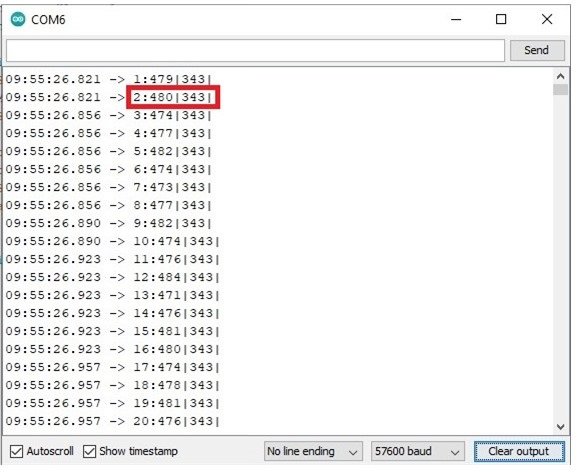
\includegraphics[width=0.7\textwidth]{img/percob/Slide1}

	(a)
	
	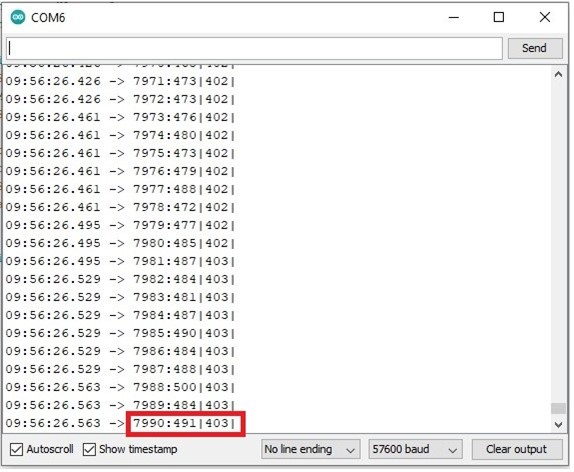
\includegraphics[width=0.7\textwidth]{img/percob/Slide2}
	
	(b)
	
	\caption{Percobaan 1 : (a)Data awal yang dikirim dari arduino, (b)Data akhir yang dikirim arduino.}
	\label{fig:4.2}
\end{figure}
\vspace{1ex}
Dapat dilihat pada Gambar \ref{fig:4.2}, tanda "$\mid$" yang ada pada data tersebut diperlukan untuk melakukan split pada program aplikasi untuk memisahkan data ECG dengan detik. Pada tanda kotak berwarna merah berisi "2:480$\mid$343$\mid$" yang mana angka "2" adalah urutan sampel dari arduino, kemudian angka "480" adalah data sensor, dan "343" merupakan detik. Pada percobaan pertama, data awal yang terkirim oleh arduino adalah 480 pada sampel ke-2 dan data terakhir yang terkirim adalah 491 pada sampel ke-7990. Apabila dihitung maka jumlah sampel yang terkirim adalah 7989 sampel dalam satu menit.
\begin{figure}[H] \centering
	\begin{subfigure}{0.45\textwidth}
		\centering
		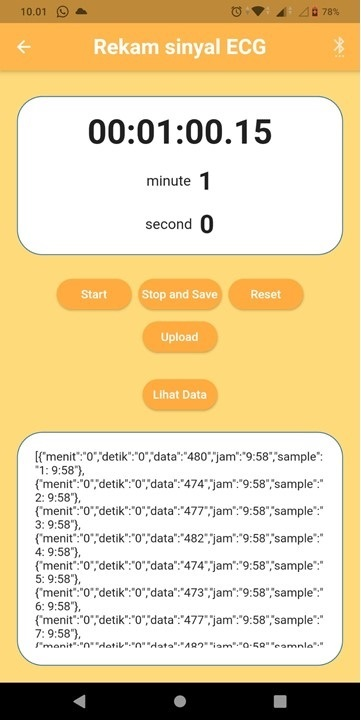
\includegraphics[width=1\linewidth]{img/percob/Slide11a}	  
		\caption{}		
	\end{subfigure}
	\begin{subfigure}{0.45\textwidth}
		\centering
		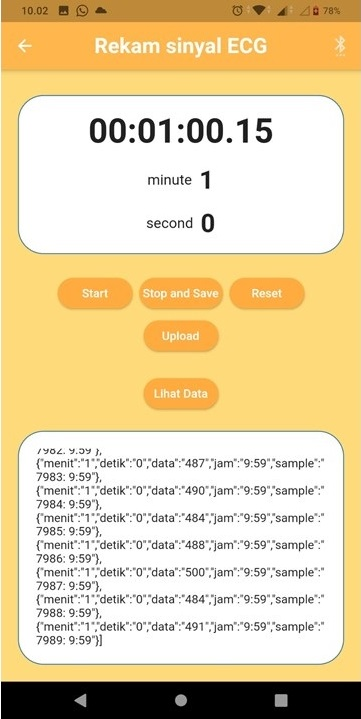
\includegraphics[width=1\linewidth]{img/percob/Slide11b.jpg}	  
		\caption{}		
	\end{subfigure}
	\caption{Percobaan 1: (a) Data awal yang diterima aplikasi, (b) Data akhir yang diterima aplikasi.}
	\label{fig:4.2.0}
\end{figure}
\vspace{1ex}
Gambar \ref{fig:4.2.0} merupakan tampilan data yang diterima aplikasi. Dapat dilihat pada gambar tersebut, data yang ada aplikasi adalah menit, detik, data, jam, dan sampel. Menit tersebut didapatkan dari memproses detik yang telah dikirim dari arduino. Detik didapatkan dari data yang dikirim oleh arduino. Data merupakan data ECG yang dikirim oleh arduino. Jam merupakan data penjumlahan antara waktu mulai rekaman dengan detik yang diperoleh dari arduino. Sampel didapat dari proses penomoran data pada aplikasi.  Layar sebelah kiri menunjukkan data pertama yang diterima adalah 480 dan layar sebelah kanan menunjukkan data terakhir yang diterima aplikasi adalah 491. Jumlah data yang diterima oleh aplikasi dapat dilihat pada nomor "sample" yaitu 7989 sampel. Berikutnya adalah gambar percobaan kedua. 
\begin{figure}[H] \centering
	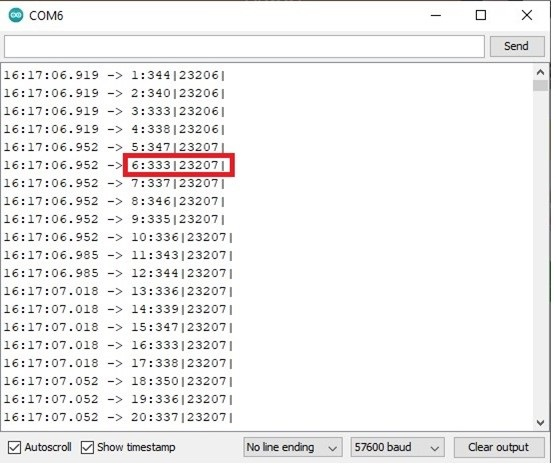
\includegraphics[width=0.7\textwidth]{img/percob/Slide3}
	
	(a)
	
	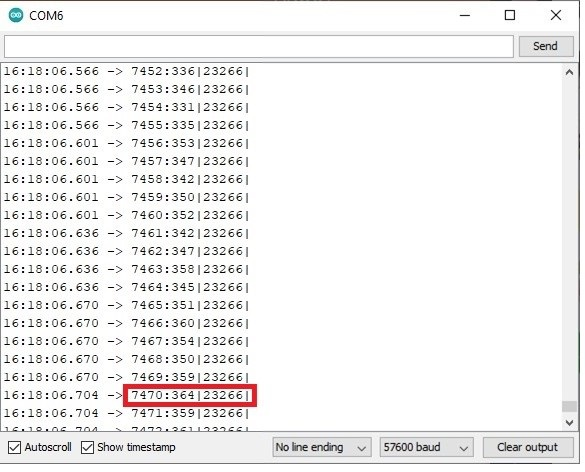
\includegraphics[width=0.7\textwidth]{img/percob/Slide4}
	
	(b)
	
	\caption{Percobaan 2 : (a)Data awal yang dikirim dari arduino, (b)Data akhir yang dikirim arduino.}
	\label{fig:4.2.1}
\end{figure}
\vspace{1ex}
Dapat dilihat pada Gambar \ref{fig:4.2.1}, pada bagian (a) data awal yang terkirim oleh arduino adalah 333 yang merupakan sampel keenam dan pada bagian (b) data terakhir yang terkirim adalah 364 yang merupakan sampel ke-7470. Jumlah data yang dikirim oleh arduino adalah 7465 sampel.

\begin{figure}[H] \centering
	\begin{subfigure}{0.45\textwidth}
		\centering
		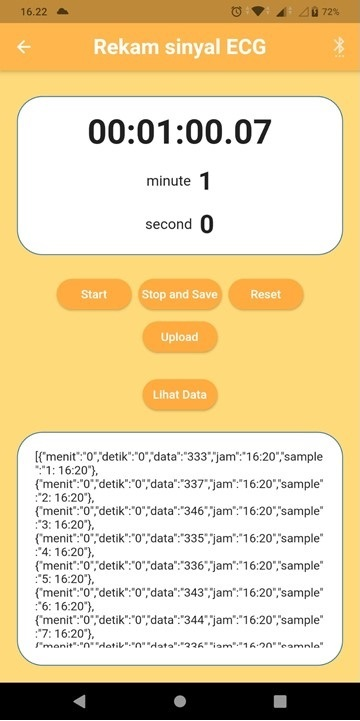
\includegraphics[width=1\linewidth]{img/percob/Slide12a}	  
		\caption{}		
	\end{subfigure}
	\begin{subfigure}{0.45\textwidth}
		\centering
		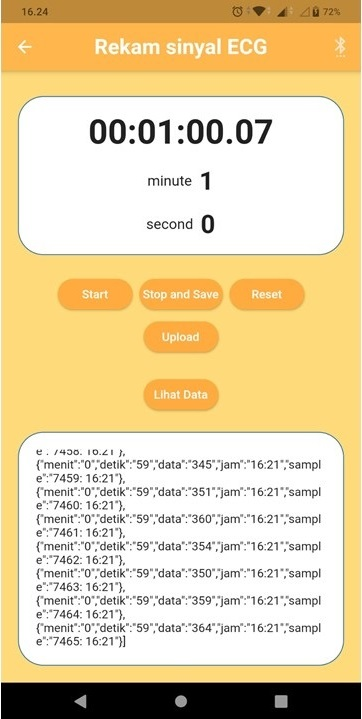
\includegraphics[width=1\linewidth]{img/percob/Slide12b.jpg}	  
		\caption{}		
	\end{subfigure}	
	\caption{Percobaan 2: (a) Data awal yang diterima aplikasi, (b) Data akhir yang diterima aplikasi.}
	\label{fig:4.2.2}
\end{figure}
\vspace{1ex}
Gambar \ref{fig:4.2.2} merupakan tampilan data yang diterima aplikasi pada percobaan kedua. Layar sebelah kiri menunjukkan data pertama yang diterima adalah 333 dan layar sebelah kanan menunjukkan data terakhir yang diterima aplikasi adalah 364. Jumlah data yang diterima oleh aplikasi dapat dilihat pada nomor "sample" yaitu 7465 sampel. Berikutnya adalah gambar percobaan ketiga. 

\begin{figure}[H] \centering
	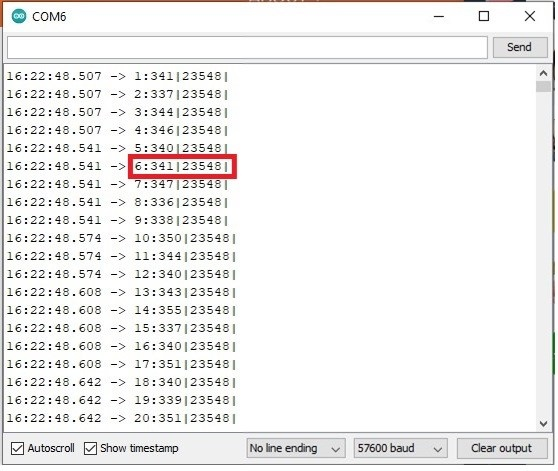
\includegraphics[width=0.7\textwidth]{img/percob/Slide5}
	
	(a)
	
	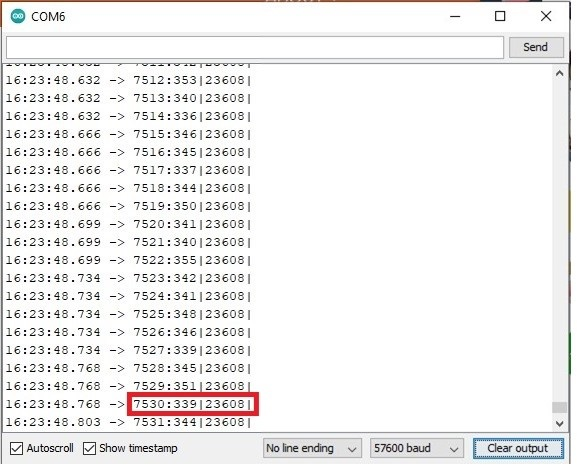
\includegraphics[width=0.7\textwidth]{img/percob/Slide6}
		
	(b)
	
	\caption{Percobaan 3 : (a)Data awal yang dikirim dari arduino, (b)Data akhir yang dikirim arduino.}
	\label{fig:4.2.3}
\end{figure}
\vspace{1ex}
Dapat dilihat pada Gambar \ref{fig:4.2.3}, pada bagian (a) data awal yang terkirim oleh arduino adalah 341 yang merupakan sampel keenam dan pada bagian (b) data terakhir yang terkirim adalah 339 yang merupakan sampel ke-7470. Jumlah data yang dikirim oleh arduino adalah 7525 sampel.

\begin{figure}[!h] \centering
	\begin{subfigure}{0.45\textwidth}
		\centering
		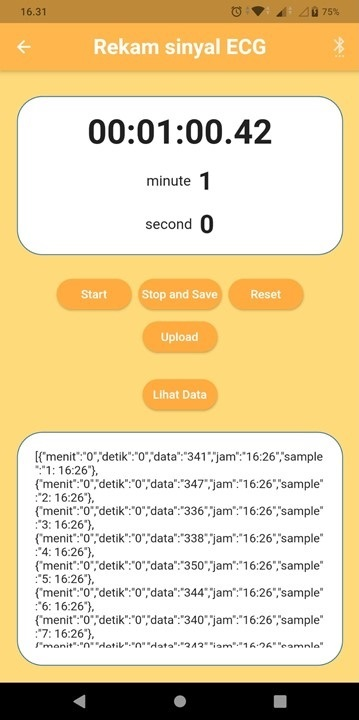
\includegraphics[width=1\linewidth]{img/percob/Slide13a}	  
		\caption{}		
	\end{subfigure}
	\begin{subfigure}{0.45\textwidth}
		\centering
		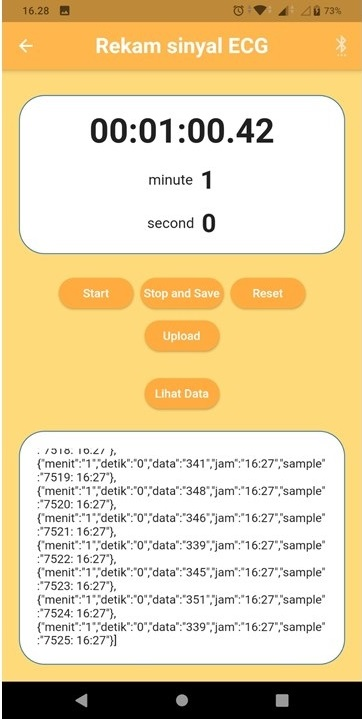
\includegraphics[width=1\linewidth]{img/percob/Slide13b.jpg}	  
		\caption{}		
	\end{subfigure}
	
	\caption{Percobaan 3: (a) Data awal yang diterima aplikasi, (b) Data akhir yang diterima aplikasi.}
	\label{fig:4.2.4}
\end{figure}
Gambar \ref{fig:4.2.4} merupakan tampilan data yang diterima aplikasi. Layar sebelah kiri menunjukkan data pertama yang diterima adalah 341 dan layar sebelah kanan menunjukkan data terakhir yang diterima aplikasi adalah 339. Jumlah data yang diterima oleh aplikasi dapat dilihat pada nomor "sample" yaitu 7525 sampel. Berikutnya adalah gambar percobaan keempat. 
\begin{figure}[H] \centering
	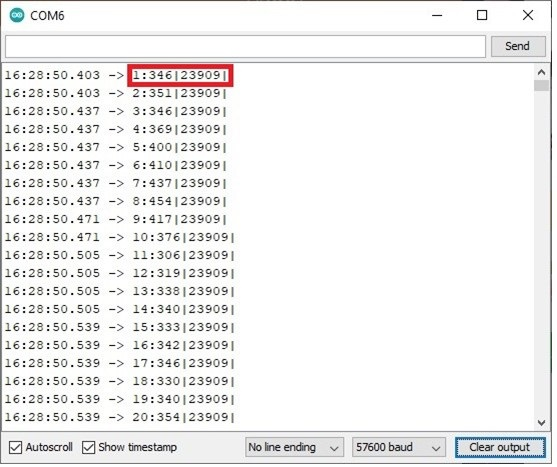
\includegraphics[width=0.7\textwidth]{img/percob/Slide7}
	
	(a)
	
	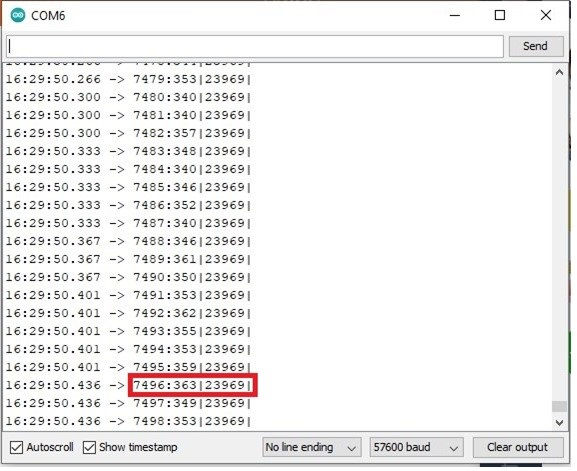
\includegraphics[width=0.7\textwidth]{img/percob/Slide8}
	
	(b)
	
	\caption{Percobaan 4 : (a)Data awal yang dikirim dari arduino, (b)Data akhir yang dikirim arduino.}
	\label{fig:4.2.5}
\end{figure}
\vspace{1ex}
Pada gambar \ref{fig:4.2.5} dapat diketahui bagian (a) data awal yang terkirim adalah 346 yang merupakan sampel pertama pada arduino, kemudian data terakhir ditampilkan pada bagian (b) yaitu 363 merupakan data urutan ke-7496 serta merupakan jumlah data yang berhasil dikirim.


\begin{figure}[H] \centering
	\begin{subfigure}{0.45\textwidth}
		\centering
		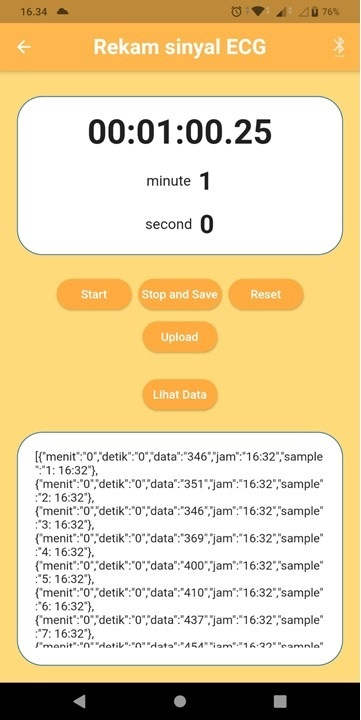
\includegraphics[width=1\linewidth]{img/percob/Slide14a}	  
		\caption{}		
	\end{subfigure}
	\begin{subfigure}{0.45\textwidth}
		\centering
		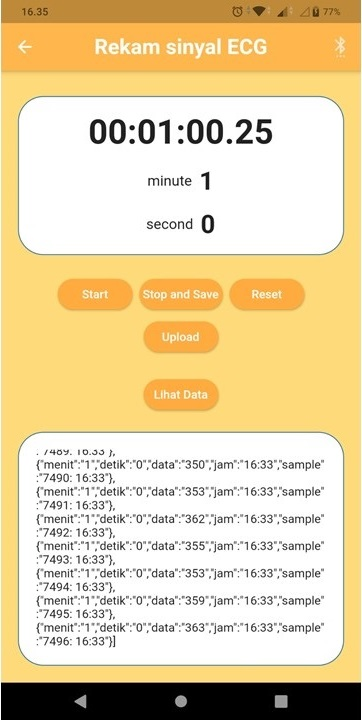
\includegraphics[width=1\linewidth]{img/percob/Slide14b.jpg}	  
		\caption{}		
	\end{subfigure}
	\caption{Percobaan 4: (a) Data awal yang diterima aplikasi, (b) Data akhir yang diterima aplikasi.}
	\label{fig:4.2.6}
\end{figure}
\vspace{1ex}
Pada percobaan keempat seperti yang diperlihatkan Gambar \ref{fig:4.2.6}, pada bagian kiri menunjukkan data awal yang diterima aplikasi yaitu 346 dan pada bagian kanan terdapat data terakhir yang diterima aplikasi yaitu 363. Jumlah data yang diterima aplikasi ditunjukkan pada nomor sampel data terakhir yaitu 7469. Kemudian berikut ini merupakan gambar percobaan terakhir.
\begin{figure}[H] \centering
	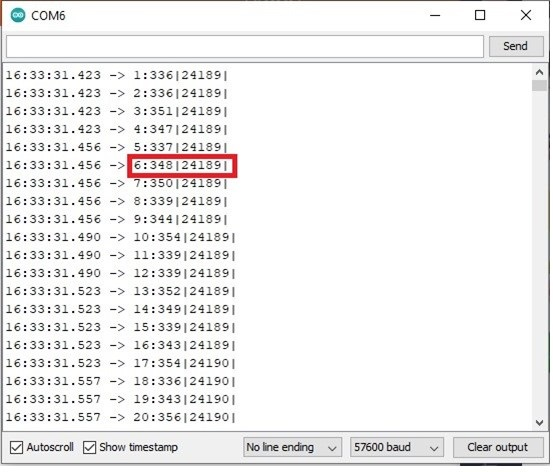
\includegraphics[width=0.7\textwidth]{img/percob/Slide9}
	
	(a)
	
	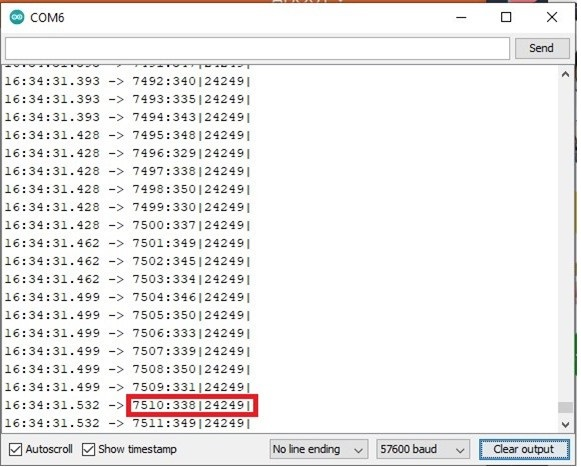
\includegraphics[width=0.7\textwidth]{img/percob/Slide10}
	
	(b)
	
	\caption{Percobaan 5 : (a)Data awal yang dikirim dari arduino, (b)Data akhir yang dikirim arduino.}
	\label{fig:4.2.7}
\end{figure}
\vspace{1ex}
Dapat diketahui dari gambar \ref{fig:4.2.7}, bagian (a) menunjukkan data awal yang terkirim yaitu 348 pada urutan sampel nomor 6, kemudian bagian (b) menunjukkan data terakhir yang terkirim yaitu 338 pada nomor sampel 7510. Apabila diperhitungkan melihat nomor sampel maka jumlah data yang terkirim adalah 7505 sampel.
\begin{figure}[H] \centering
	\begin{subfigure}{0.45\textwidth}
		\centering
		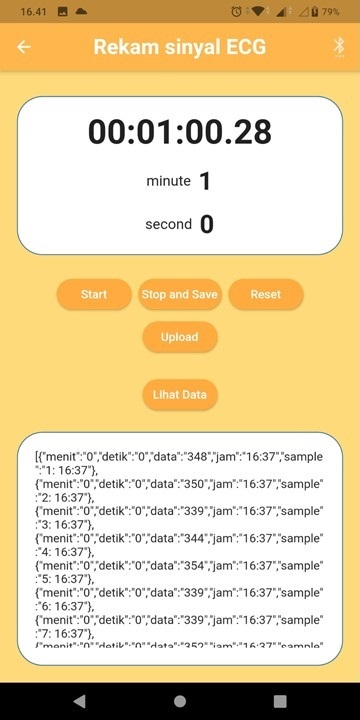
\includegraphics[width=1\linewidth]{img/percob/Slide15a}	  
		\caption{}		
	\end{subfigure}
	\begin{subfigure}{0.45\textwidth}
		\centering
		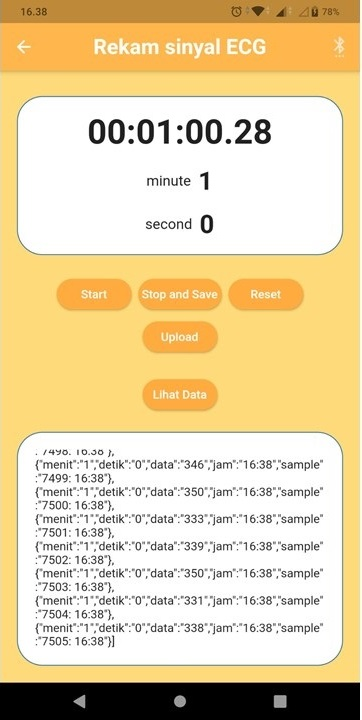
\includegraphics[width=1\linewidth]{img/percob/Slide15b.jpg}	  
		\caption{}		
	\end{subfigure}
	\caption{Percobaan 5: (a) Data awal yang diterima aplikasi, (b) Data akhir yang diterima aplikasi.}
	\label{fig:4.2.8}
\end{figure}
Pada percobaan terakhir didapatkan data seperti yang diperlihatkan Gambar \ref{fig:4.2.8}, pada bagian kiri menunjukkan data awal yang diterima aplikasi yaitu 348 dan pada bagian kanan terdapat data terakhir yang diterima aplikasi yaitu 338. Jumlah data yang diterima aplikasi ditunjukkan pada nomor sampel data terakhir yaitu 7505 sehingga jumlah data yang dikirim arduino sesuai dengan jumlah data yang diterima aplikasi. Untuk lebih jelasnya dapat dilihat pada tabel berikut.

\begin{table}[H]
	\begin{tabular}{|c|c|c|c|c|c|}
		\hline
		\multirow{3}{*}{\textbf{Uji ke-}} & \multicolumn{3}{|c|}{\textbf{Arduino}}& \multicolumn{1}{|c|}{\textbf{Aplikasi}}&
		\multicolumn{1}{|c|}{\textbf{Sesuai}}\\
		\cline{2-5} & \textbf{Nomor} & \textbf{Nomor} & \textbf{Jumlah}&\textbf{Jumlah} &  \\
		 & \textbf{sampel} & \textbf{sampel} & \textbf{sampel}& \textbf{sampel}&\\
		 &\textbf{awal}&\textbf{akhir}&&\textbf{diterima}&\\
		\hline1& 2 &7990 & 7989&7989&ya\\
		\hline2&6&7470&7465&7465 &ya  \\
		\hline3&6 &7530 &7525&7525&ya \\
		\hline4&1 &7496 &7496&7496&ya \\
		\hline3&6 &7510 &7505&7505&ya \\
		\hline
	\end{tabular}
\end{table}

\section{Pengujian Persentase Data Hilang}
\vspace{1ex}
Pada bagian ini, pengujian dilakukan dengan cara merekam data ECG yang dikirimkan oleh arduino. Pada pengujian ini menggunakan \textit{baudrate} sebesar 9600. Pengujian ini dilakukan untuk mengetahui seberapa banyak data yang hilang dengan cara membandingkan data yang dikirim oleh mikrokontroler arduino dengan data yang diterima oleh aplikasi. Berikut adalah tabel yang merupakan hasil percobaan selama 1 menit (Tabel \ref{tabel:4.1}).



\begin{table}[H]
	\caption{Tabel hasil percobaan persentase data hilang}
	\begin{tabular}{|c|c|c|c|c|c|}
		\hline
		\multicolumn{1}{|c|}{{\color[HTML]{000000} \textbf{Delay}}} & \multicolumn{1}{|c|}{\textbf{Uji}} &
		\multicolumn{1}{|c|}{ \textbf{Jumlah}} &
		\multicolumn{1}{|c|}{\textbf{Jumlah}} &
		\multicolumn{1}{|c|}{\textbf{\textit{Sampling}}}  & 
		\multicolumn{1}{|c|}{\textbf{Data}} \\
		(ms) &  \textbf{ke-}  & \textbf{rekaman}  & \textbf{data} & \textbf{\textit{rate}}  & \textit{hilang}\\
		&  &  &  \textbf{diterima} & & (\%) \\ \hline
		
		\multirow{5}{*}{5} &1& 15:00.09 &118317 &131 & 0.33 \\
		\cline{2-6}&2 &15.00.55 & 118214 &131 & 0.26\\ 
		\cline{2-6}&3 &15.00.73 & 118235 &131 & 0.33\\ 
		\cline{2-6}&4 &15.01.75 & 118229 &131 & 0.20\\ 
		\cline{2-6}&5 &15.00.34 & 118143 &131 & 0.18\\ 
		\hline
		\multirow{5}{*}{3} &1& 15:00.49 &161161 &179 & 0.24 \\
		\cline{2-6}&2 &15.14.86 & 162735 &180 & 0.32\\ 
		\cline{2-6}&3 &15.00.65 & 160370 &178 & 0.28\\ 
		\cline{2-6}&4 &15.00.54 & 161134 &179 & 0.31\\ 
		\cline{2-6}&5 &15.00.76 & 161743 &179 & 0.36\\ 
		\hline
		
	\end{tabular}
	\vspace{1ex}
	
	\label{tabel:4.1}
\end{table}
Tabel \ref{tabel:4.1} merupakan tabel yang memiliki 6 kolom yaitu Delay, Uji ke-, Jumlah Data dikirim, Jumlah Data diterima, Sampling
rate, Data hilang. Delay merupakan durasi jeda waktu pada loop
arduino. Jumlah Data dikirim merupakan banyak data yang dikirim
oleh arduino menuju aplikasi. Jumlah Data diterima merupakan banyak data yang telah sampai di aplikasi. \textit{Sampling rate} merupakan
banyak data yang diterima aplikasi pada setiap detik. Data hilang
merupakan jumlah data yang tidak berhasil sampai pada aplikasi.



Pada tabel \ref{tabel:4.1} terdapat kolom \textit{sampling rate} yang mana merupakan jumlah sample yang berhasil diterima oleh aplikasi dalam 1
detik. Perhitungan \textit{sampling rate} dengan cara perbandingan antara
jumlah data diterima dengan waktu uji. Selain itu juga terdapat
kolom data hilang dimana merupakan persentase jumlah data yang
tidak berhasil diterima oleh aplikasi. Perhitungan persentase data hilang adalah dengan cara membandingkan selisih jumlah data
dikirim dengan jumlah data diterima dengan jumlah data dikirim
kemudian dikalikan dengan 100 \%. Dari tabel 4.7 didapatkan persentasi data yang hilang adalah dibawah 1\%.

\vspace{1ex}


\section{Pengujian Kesesuian Grafik ECG}
\vspace{1ex}

Pada tahap ini, dilakukan pengujian dengan cara membandingkan grafik ECG yang telah ditampilkan oleh aplikasi android dengan grafik ECG yang ditampilkan oleh serial ploter yang merupakan tools dari Arduino IDE. Berikut adalah hasil grafik ECG yang ditampilkan oleh aplikasi Gambar \ref{fig:4.0}.

\begin{figure}[H] \centering
	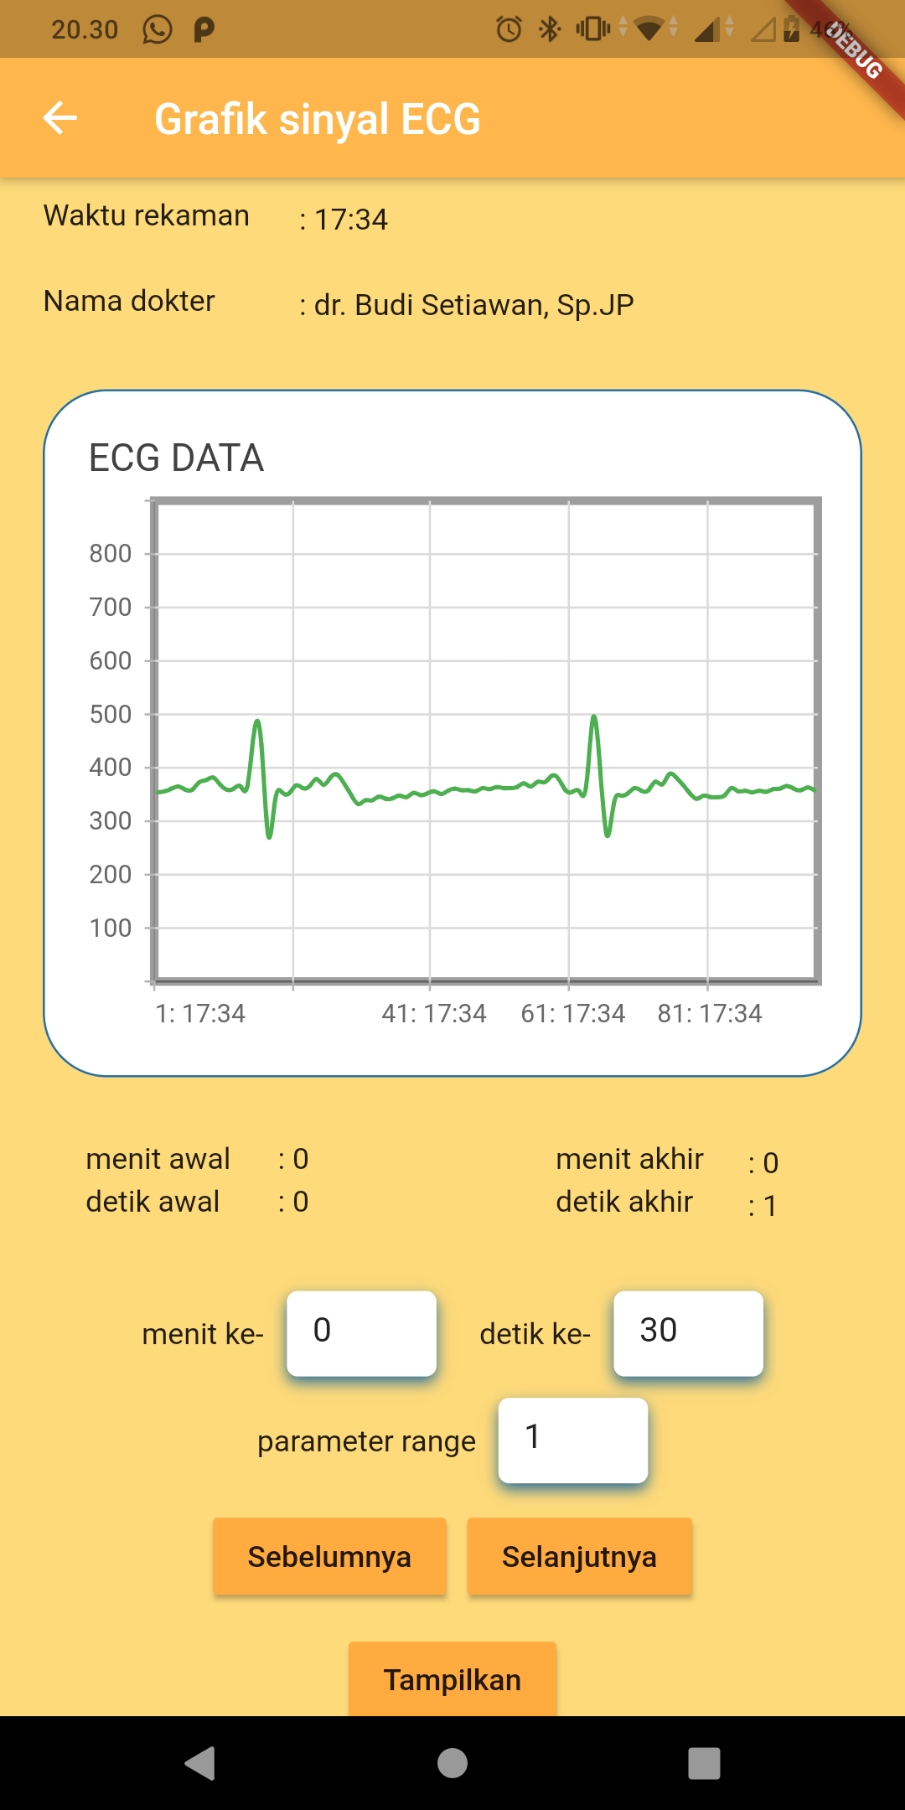
\includegraphics[width=0.45\textwidth]{img/grafikECGapps.jpg}
	\caption{Grafik ECG yang ditampilkan pada aplikasi.}
	\label{fig:4.0}
\end{figure}
Sedangkan grafik ECG yang ditampilkan pada serial ploter Arduino IDE ditunjukkan pada gambar berikut.
\begin{figure}[H] \centering
	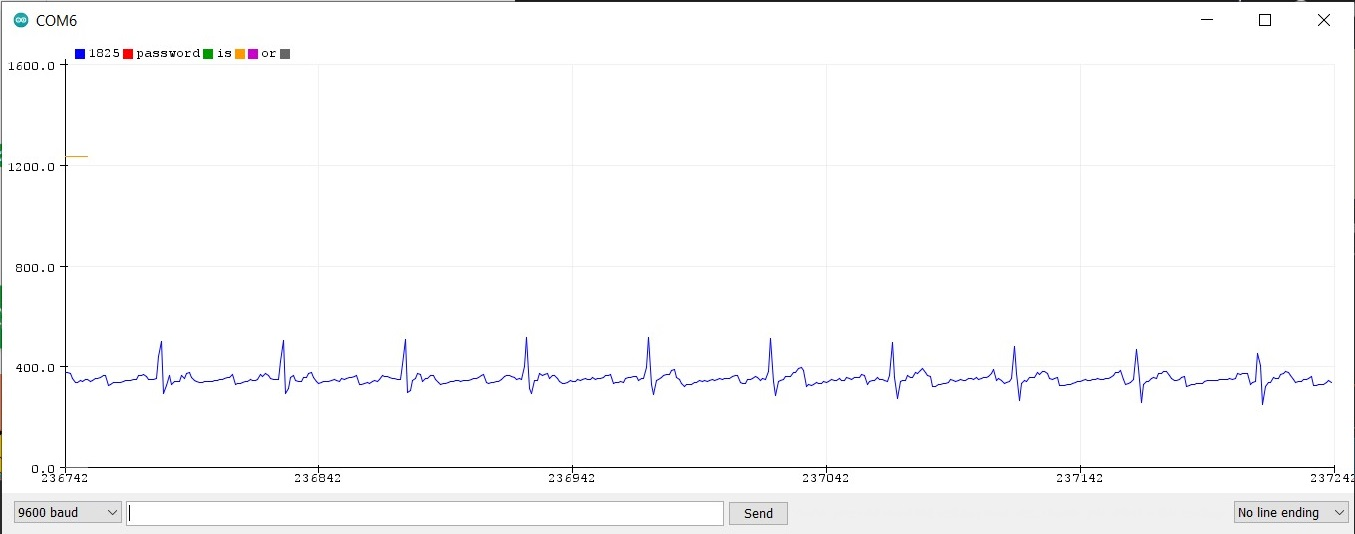
\includegraphics[width=1\textwidth]{img/ujisesuaidataIDE.jpg}
	\caption{Grafik ECG yang ditampilkan pada serial ploter Arduino IDE.}
	\label{fig:4.1}
\end{figure}

Berdasarkan kedua gambar diatas, apabila dibandingkan maka kedua gambar tersebut cukup mirip. Dengan demikian berarti hasil grafik ECG yang ditampilkan oleh aplikasi android cukup sesuai dengan grafik ECG yang ditampilkan oleh serial ploter Arduino IDE.
\vspace{1ex}

